\documentclass[letterpaper,11pt,nointlimits,reqno]{amsart}
\pagestyle{headings}

% Packages
\usepackage{accents}
\usepackage{array}
\usepackage{booktabs}
\usepackage{caption}
\usepackage{enumerate}
\usepackage{fancyhdr}
\usepackage[final]{graphicx}
\usepackage{fullpage}
\usepackage{lastpage}
\usepackage{listings}
\usepackage{longtable}
\usepackage{mathrsfs}
\usepackage{mathtools}
\usepackage[numbers,sort&compress]{natbib}
\usepackage[usenames,dvipsnames,svgnames,table]{xcolor}

% Avoids xcolor options clashes
\usepackage{pgfplotstable}

% In conjunction with -shell-escape, automatically convert EPS to PDF
\usepackage{epstopdf}
\epstopdfsetup{outdir=./,suffix=-generated,update,verbose}
\epstopdfDeclareGraphicsRule{.eps}{pdf}{.pdf}{%
    epstopdf --outfile=\OutputFile \space `kpsewhich \space "\SourceFile"`
}

% Hyperref package must be last otherwise the contents are jumbled
% hypertexnames disabled to fix links pointing to incorrect locations
\usepackage[hypertexnames=false,final]{hyperref}

\mathtoolsset{showonlyrefs,showmanualtags}
% \allowdisplaybreaks[1] % Allow grouped equations to be split across pages

% Document-specific commands
\newcommand{\Mach}[1][]{\mbox{Ma}_{#1}}

% From how-to-prevent-a-page-break-before-an-itemize-list
% http://tex.stackexchange.com/questions/2644
\makeatletter
\newcommand\mynobreakpar{\par\nobreak\@afterheading}
\makeatother

% Configure inline code listings
\lstset{
  basicstyle=\footnotesize\sffamily,
  columns=fixed,
  commentstyle=\color{blue},
  firstnumber=1,
  frame=single,
  keepspaces=true,
  numberfirstline=true,
  numbersep=7pt,
  numbers=left,
  numberstyle=\tiny\color{darkgray},
  showstringspaces=false,
  showtabs=false,
  stepnumber=5
}

\begin{document}

\title{Favorable pressure gradient base flow computations}
\author{Rhys Ulerich}

\begin{abstract}
This document discusses how to obtain a favorable pressure gradient base flow
for use within temporally homogenized boundary layer simulations.  First, a
compressible potential flow problem is formulated for an isenthalpic, radially
symmetric source or sink flow.  The resulting one-dimensional problem is cast
into a form commodity ODE integrators can solve to obtain primitive state as a
function of radius.  The solution is then mapped from $\left(r,\theta\right)$
into $\left(x,y\right)$ coordinates and a base flow profile extracted from some
constant $x$ line segment.  The segment chosen, as well as the radial problem
boundary conditions used, are taken to match some boundary layer edge state of
interest.  Finally, this procedure is used to produce base flows in the spirit
of laminar CEV heat shield conditions.
\end{abstract}

\maketitle

\tableofcontents

%%%%%%%%%%%%%%%%%%%%%%%%%%%%%%%%%%%%%%%%%%%%%%%%%%%%%%%%%%%%%%%%%%%%%%%%%%%%%%%
\section{The nondimensional, compressible, isenthalpic potential flow equation}
%%%%%%%%%%%%%%%%%%%%%%%%%%%%%%%%%%%%%%%%%%%%%%%%%%%%%%%%%%%%%%%%%%%%%%%%%%%%%%%

A succinct, coordinate-independent derivation of the velocity-potential
formulation of the compressible potential flow equations appears in section
II.A of \citet{Saad2011Coordinate}.  Their presentation essentially is
recounted here but velocity potential notation is suppressed.  Wherever
necessary, sufficient smoothness is assumed.

The steady, inviscid momentum equation in an irrotational flow yields
\begin{align}
    \vec{\nabla}p
    &= -\rho \vec{u}\cdot\vec{\nabla}\vec{u}
     = -\rho \left(   \frac{1}{2}\vec{\nabla}\left(\vec{u}\cdot\vec{u}\right)
                    - \vec{u}\times\vec{\nabla}\times\vec{u}
        \right)
     = - \frac{1}{2} \rho \vec{\nabla}\vec{u}^2
\label{eq:momentum}
.
\end{align}
The irrotational velocity may be replaced by the gradient of a scalar
potential, \emph{viz.}
\begin{align}
  \vec{u} = \vec{\nabla}\phi + \vec{\nabla}\times\vec{A} = \vec{\nabla}{\phi}
  .
\end{align}
Combining the definition of the speed of sound~$a$
and equation~\eqref{eq:momentum},
\begin{align}
    \left(\frac{\partial p}{\partial \rho}\right)_{s} = a^2
    \implies
    \vec{\nabla}\rho = \frac{1}{a^2} \vec{\nabla} p
                     = - \frac{\rho}{2a^2} \vec{\nabla}\vec{u}^2
\label{eq:gradrho_gradp_relationship}
.
\end{align}
Expanding the steady continuity equation and
applying~\eqref{eq:gradrho_gradp_relationship},
\begin{align}
  0 &= \vec{\nabla}\cdot\rho\vec{u}
     = \rho\vec{\nabla}\cdot\vec{u} + \vec{u}\cdot\vec{\nabla}\rho
     = \rho\vec{\nabla}\cdot\vec{u}
     - \frac{\rho\vec{u}}{2a^2} \cdot \vec{\nabla}\vec{u}^2
\label{eq:continuity}
.
\end{align}
Because $\rho>0$ and $a>0$, for nontrivial $\vec{u}$ the above
equation may only be satisfied when
\begin{align}
       \frac{1}{2} \vec{u}\cdot \vec{\nabla}\vec{u}^2
    &= a^2 \vec{\nabla}\cdot\vec{u}
.
\label{eq:momentum_and_continuity}
\end{align}

Following \citeauthor{Saad2011Coordinate}, the specific total enthalpy is
assumed to be invariant through the flow to connect $a$ and $u$ with a
reference specific enthalpy $h_0 = a_0^2 / \left(\gamma_0-1\right)$ and
reference velocity $u_0$.  That is,
\begin{align}
     H
     &=
        \frac{a^2  }{\gamma  -1} + \frac{1}{2} \vec{u}^2
      = \frac{a_0^2}{\gamma_0-1} + \frac{1}{2} u_0^2
      =  H_0
\end{align}
holds everywhere.  After a slight rearrangement, our constant stagnation
condition
\begin{align}
        a^2
     &=   \frac{\gamma-1}{\gamma_0-1} a_0^2
        + \frac{\gamma-1}{2} \left(u_0^2 - \vec{u}^2\right)
\label{eq:stagnation_sound}
\end{align}
may be used within equation \eqref{eq:momentum_and_continuity} to obtain
\begin{align}
       \vec{u}\cdot \vec{\nabla}\vec{u}^2
    &= \left[
          2 \frac{\gamma-1}{\gamma_0-1} a_0^2
        + \left(\gamma-1\right) \left(u_0^2 - \vec{u}^2\right)
       \right]\vec{\nabla}\cdot\vec{u}
.
\end{align}
Adding a constant $\gamma=\gamma_0$ assumption, one finds the dimensional result
\begin{align}
       \vec{u}\cdot \vec{\nabla}\vec{u}^2
    &= \left[
          2 a_0^2
        + \left(\gamma_0-1\right) \left(u_0^2 - \vec{u}^2\right)
       \right]\vec{\nabla}\cdot\vec{u}
\label{eq:cpfgibbs_dim}
.
\end{align}

To nondimensionalize, choose some reference length $l_0$ and declare
\begin{align}
    x     &= x^\ast l_0
&   a     &= a^\ast a_0
&   u     &= u^\ast u_0 = u^\ast \Mach[0] a_0
&   \rho  &= \rho^\ast \rho_0
&   p     &= p^\ast \rho_0 a_0^2
\label{eq:nondimensionalization}
\end{align}
where the starred quantities are dimensionless.  Inserting these definitions
into~\eqref{eq:cpfgibbs_dim},
\begin{align}
       \frac{\Mach[0]{}^3 a_0^3}{l_0}
       \,
       \vec{u}^\ast \cdot \vec{\nabla}^\ast{\vec{u}^\ast}^2
    &=
       \left[
          2 a_0^2
        + \Mach[0]{}^2 a_0^2 \left(\gamma_0-1\right) \left(1 - {\vec{u}^\ast}^2\right)
       \right]
       \,
       \frac{\Mach[0]{} a_0}{l_0}
       \,
       \vec{\nabla}^\ast\cdot\vec{u}^\ast
\\
    &=
       \frac{\Mach[0]{}^3 a_0^3}{l_0}
       \,
       \left[
          \frac{2}{\Mach[0]{}^2}
        + \left(\gamma_0-1\right) \left(1 - {\vec{u}^\ast}^2\right)
       \right]
       \vec{\nabla}^\ast\cdot\vec{u}^\ast
.
\end{align}
Rescaling and dropping the star notation, one finally arrives at
\begin{align}
       \vec{u} \cdot \vec{\nabla}\vec{u}^2
    &=
       \left[
          2 \Mach[0]{}^{-2}
        + \left(\gamma_0-1\right) \left(1 - \vec{u}^2\right)
       \right]
       \vec{\nabla}\cdot\vec{u}
\label{eq:cpfgibbs_nondim}
.
\end{align}

With some $\vec{u}=\vec{\nabla}\phi$ satisfying~\eqref{eq:cpfgibbs_nondim} in
hand, computing local $\rho$ and $p$ is often of interest.
Nondimensionalizing~\eqref{eq:stagnation_sound} when $\gamma=\gamma_0$ permits
direct computation of $a$ from
\begin{align}
  a^2 &= 1 + \Mach[0]^2\frac{\gamma_0-1}{2}\left(1-\vec{u}^2\right)
\label{eq:stagnation_sound_nondim}
\end{align}
where clearly a realizable $a^2>0$ requires
\begin{align}
  u^2 &< \frac{2}{\Mach[0]^2\left(\gamma_0-1\right)} + 1
.
\label{eq:stagnation_sound_realizability_nondim}
\end{align}
Employing~\eqref{eq:gradrho_gradp_relationship},
nondimensionalizing, multiplying by $l_0$, and simplifying,
\begin{align}
  \frac{\vec{\nabla}\rho}{\rho}
  =
  \vec{\nabla}\log\rho
  &=
  -\frac{\Mach[0]^2}{2}\frac{\vec{\nabla}\vec{u}^2}{a^2}
.
\end{align}
Nondimensionalizing the momentum result~\eqref{eq:momentum} and then scaling by
$\frac{l_0}{\rho_0 a_0^2}$,
\begin{align}
  \vec{\nabla} p &= - \frac{1}{2}\Mach[0]^2 \rho \vec{\nabla}\vec{u}^2
.
\end{align}
Both of the previous two local statements can be made global by integrating
over some domain $\Omega$ and applying a corollary of Gauss' theorem:
\begin{align}
  \int_{\partial\Omega} \log\rho \, \mathrm{d}S
  &=
  - \frac{\Mach[0]^2}{2}\int_{\Omega}
    \frac{\vec{\nabla}\vec{u}^2}{a^2} \, \mathrm{d}x
\label{eq:logrho_nondim}
\\
  \int_{\partial\Omega} p \, \mathrm{d}S
  &=
  - \frac{\Mach[0]^2}{2}\int_{\Omega} \rho \vec{\nabla}\vec{u}^2 \, \mathrm{d}x
\label{eq:p_nondim}
\end{align}

%%%%%%%%%%%%%%%%%%%%%%%%%%%%%%%%%%%%%%%%%%%%%%%%%%%%%%%%%%%%%%%%%%%%%%%%%%%%%%%%
\section{Reduction to the radially symmetric, two-dimensional case}
%%%%%%%%%%%%%%%%%%%%%%%%%%%%%%%%%%%%%%%%%%%%%%%%%%%%%%%%%%%%%%%%%%%%%%%%%%%%%%%%

Suppose a two-dimensional domain possessing radial symmetry in which
$\vec{u}={u}\!\left(r\right)\hat{r}$.  Then the velocity potential
$\vec{\nabla}\phi$ is superfluous and~\eqref{eq:cpfgibbs_nondim} is nothing but
the scalar equation
\begin{align}
       2 u^2\!\left(r\right) u^\prime\!\left(r\right)
    &=
       \left[
          2 \Mach[0]{}^{-2}
        + \left(\gamma_0-1\right) \left(1 - u^2\!\left(r\right)\right)
       \right]
       \left(
          r^{-1} u\!\left(r\right) + u^\prime\!\left(r\right)
       \right)
.
\end{align}
Suppressing the dependence of $u$ on $r$ and collecting $u^\prime$ terms,
\begin{align}
       \left(
           2 u^2
         - \left[
              2 \Mach[0]{}^{-2} + \left(\gamma_0-1\right) \left(1 - u^2\right)
           \right]
       \right)
       u^\prime
    &=
       \left[
          2 \Mach[0]{}^{-2} + \left(\gamma_0-1\right) \left(1 - u^2\right)
       \right]
       r^{-1} u
.
\end{align}
Solving for $u^\prime$,
\begin{align}
       u^\prime
    &=
       \frac{u}{r}
       \,
       \frac{
         \left[
            2 \Mach[0]{}^{-2} + \left(\gamma_0-1\right) \left(1 - u^2\right)
         \right]
       }{
           2 u^2
         - \left[
              2 \Mach[0]{}^{-2} + \left(\gamma_0-1\right) \left(1 - u^2\right)
           \right]
       }
\label{eq:cpfradial_nondim_ode}
,
\end{align}
permits integrating $u$ given a boundary condition on either $R_1$ or $R_2$.

Given some $u$, computing local thermodynamic state also is of interest.
Equation~\eqref{eq:stagnation_sound_nondim} fixes~$a$.  The
$u=u\!\left(r\right)$ assumption reduces~\eqref{eq:logrho_nondim} to
\begin{align}
  \rho\!\left(R_2\right)
  &=
  \exp\left[
    - \frac{\Mach[0]^2}{2} \int_{R_1}^{R_2}
        \frac{\left(u^2\right)'}{a^2}
      \, r \, \mathrm{d}r
    + \log\rho\!\left(R_1\right)
  \right]
   =
  \rho\!\left(R_1\right) \exp\left[
    - \Mach[0]^2 \int_{R_1}^{R_2}
        \frac{u u'}{a^2}
      \, r \, \mathrm{d}r
  \right]
\label{eq:cpfradial_nondim_rho}
\end{align}
where the $2\pi$ factors arising from integrating cancel each other.
Likewise~\eqref{eq:p_nondim} simplifies to
\begin{align}
  p\!\left(R_2\right)
  &=
    - \frac{\Mach[0]^2}{2} \int_{R_1}^{R_2}
        \rho \left(u'\right)^2
      \, r \, \mathrm{d}r
    + p\!\left(R_1\right)
   =
    -\Mach[0]^2 \int_{R_1}^{R_2} \rho u u' \, r \, \mathrm{d}r
      + p\!\left(R_1\right)
\label{eq:cpfradial_nondim_p}
.
\end{align}
Notice~\eqref{eq:cpfradial_nondim_ode} easily supplies pointwise $u'$ for the
computation of both $\rho$ and $p$.

%%%%%%%%%%%%%%%%%%%%%%%%%%%%%%%%%%%%%%%%%%%%%%%%%%%%%%%%%%%%%%%%%%%%%%%%%%%%%%%%
\section{The sub- and supersonic radial nozzle problems}
%%%%%%%%%%%%%%%%%%%%%%%%%%%%%%%%%%%%%%%%%%%%%%%%%%%%%%%%%%%%%%%%%%%%%%%%%%%%%%%%

Equations~\eqref{eq:stagnation_sound_nondim}, \eqref{eq:cpfradial_nondim_ode},
\eqref{eq:cpfradial_nondim_rho} and~\eqref{eq:cpfradial_nondim_p} may be used
to find nondimensional solutions to idealized sub- and supersonic radial nozzle
and diffuser problems. Many texts, e.g.
\citet[\textsection{}9.4]{White1999Fluid} and
\citet[\textsection{}97]{Landau2004Fluid}, discuss the situation when the
nozzle area changes slowly as one progresses downstream in the device.  In
contrast, the preceding treatment permits geometries violating that assumption.

A subsonic nozzle may be posed on nondimensional~$\left[R_{1}, R_{2}\right]$ by
setting inflow per
\begin{align}
    -a_0 < u\!\left(l_0 R_{2}\right) u_0 < 0
    &\implies
    u\!\left(R_{2}\right) \in \left(-\Mach[0]^{-1}, 0\right)
.
\end{align}
With this inflow, $-u$ increases and $p$ decreases when traversing the
domain from~$R_{2}$ to~$R_{1}$.  However, not surprisingly, the problem becomes
stiff as the flow accelerates towards sonic conditions.  A workaround is
specifying at most a sonic outflow via
\begin{align}
    -a_0 < u_0 u\!\left(l_0 R_1\right) < 0
    &\implies
    u\!\left(R_1\right) \in \left(-\Mach[0]^{-1}, 0\right)
\end{align}
in conjunction with taking $R_{2}$ large enough to obtain the desired upstream
$u\!\left(R_{2}\right)$ condition.  Further incorporating
realizability~\eqref{eq:stagnation_sound_realizability_nondim} taking care to
use the negative square root of $u^2$ shows
\begin{align}
  \max\left(
    -\frac{1}{\Mach[0]}, -\sqrt{\frac{2}{\Mach[0]^2\left(\gamma_0-1\right)}+1}
  \right) < &u\!\left(R_1\right) < 0
\label{eq:cpfradial_nozzle_subsonic_bc}
\end{align}
is required.  Caveat numerical errors, specifying either the inflow or outflow
condition is equivalent as the physics are frictionless.

A supersonic nozzle may be posed on nondimensional~$\left[R_{1}, R_{2}\right]$
by setting inflow
\begin{align}
   u_0 u\!\left(l_0 R_{1}\right) > a_0 > 0
   &\implies
   u\!\left(R_{1}\right) \in \left(\Mach[0]^{-1}, \infty\right)
.
\end{align}
Again incorporating
realizability~\eqref{eq:stagnation_sound_realizability_nondim} via the positive
square root of $u^2$,
\begin{align}
  \frac{1}{\Mach[0]} < &u\!\left(R_1\right)
  < \sqrt{\frac{2}{\Mach[0]^2\left(\gamma_0-1\right)}+1}
\label{eq:cpfradial_nozzle_supersonic_bc}
.
\end{align}
With this inflow, $u$ increases and $p$ decreases when traversing the domain
from~$R_{1}$ to~$R_{2}$.  As above, a supersonic outflow could instead be
specified at $R_{2}$.

Working with conditions~\eqref{eq:cpfradial_nozzle_subsonic_bc}
and~\eqref{eq:cpfradial_nozzle_supersonic_bc} on $\left[R_1, R_2\right]$ in
conjunction with~\eqref{eq:cpfradial_nondim_ode} presents initial value
problems amenable to solution by numerical ODE integrators.  For example,
\texttt{Octave}\citep{Eaton2008GNU} armed with the \texttt{odepkg} package can
solve such problems.  One possible implementation appears in
Listing~\ref{lst:octave_nozzle} with verification tests.  Its demo logic
produces the solutions depicted in Figure~\ref{fig:sample_solns}.  Though only
scalar $u^\prime\!\left(r\right)$ needs to be integrated, this implementation
integrates the state vector $\left[u, \rho, p\right]^\mathrm{T}$ so that
\texttt{odepkg}'s automated solution tolerance controls apply equally to all
three quantities.

\lstinputlisting[language=Octave,label=lst:octave_nozzle,
                 caption={\texttt{nozzle.m}: A nondimensional
                 radial flow solver implementation}]
                {notebooks/nozzle.m}

\begin{figure}[p]
  \centering
  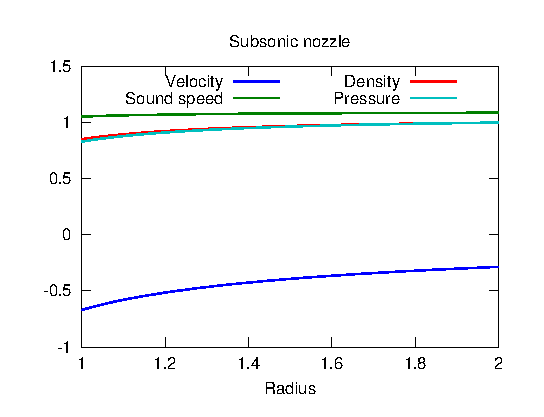
\includegraphics[width=0.80\textwidth]{nozzle_subsonic}
  \vfill
  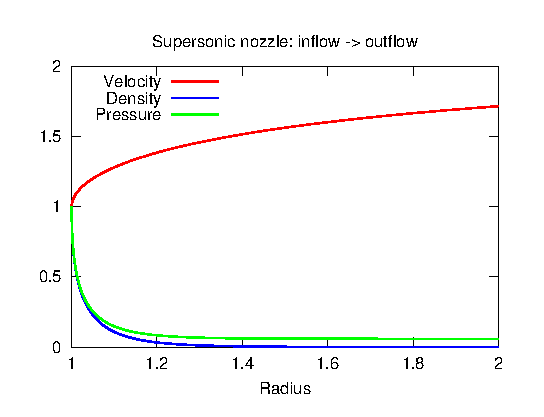
\includegraphics[width=0.80\textwidth]{nozzle_supersonic}
  \caption{
      \label{fig:sample_solns}
      Sample solutions saved by the demo logic in \texttt{nozzle.m}.  The
      subsonic case flows from right-to-left while the supersonic one flows
      from left-to-right.
  }
\end{figure}

\clearpage

%%%%%%%%%%%%%%%%%%%%%%%%%%%%%%%%%%%%%%%%%%%%%%%%%%%%%%%%%%%%%%%%%%%%%%%%%%%%%%%%
\section{Computing quantities of interest for a Cartesian base flow}
%%%%%%%%%%%%%%%%%%%%%%%%%%%%%%%%%%%%%%%%%%%%%%%%%%%%%%%%%%%%%%%%%%%%%%%%%%%%%%%%

\begin{figure}[h]
  \centering
  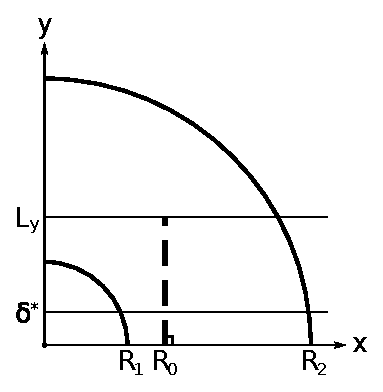
\includegraphics[width=0.33\textwidth]{nozzle_schematic}
  \caption{
      \label{fig:mapping_geometry}
      A Cartesian setting overlaid on the radially symmetric domain
  }
\end{figure}
%
Suppose a Cartesian flow profile of height $L_y$ is desired from a constant $x$
line segment within a radially varying solution.
Referring to Figure~\eqref{fig:mapping_geometry}, assume a solution
$u\!\left(R\right)$ with accompanying $\rho\!\left(R\right)$,
$p\!\left(R\right)$, and $a\!\left(R\right)$ is valid for any
$R\in\left[R_1,R_2\right]$.  Then for some $\left(x,y\right)$ and corresponding
$R=\sqrt{x^2+y^2}$ one may compute the following:
%
\begin{align}
              \rho \!\left(x, y\right)        &= \rho\!\left(R\right)
 & \partial_x \rho                            &= \frac{x}{R} \rho^\prime\!\left(R\right)
 & \partial_y \rho                            &= \frac{y}{R} \rho^\prime\!\left(R\right)
\\            u_x  \!\left(x, y\right)        &= u   \!\left(R\right) \frac{x}{R}
 & \partial_x u_x                             &= \frac{1}{R^2}\left[x^2 u^\prime\!\left(R\right) + \frac{y^2}{R} u\!\left(R\right)\right]
 & \partial_y u_x                             &= \frac{xy}{R^2}\left[u^\prime\!\left(R\right) - \frac{1}{R}u\!\left(R\right)\right]
\\            u_y  \!\left(x, y\right)        &= u   \!\left(R\right) \frac{y}{R}
 & \partial_x u_y                             &= \frac{xy}{R^2}\left[u^\prime\!\left(R\right) - \frac{1}{R}u\!\left(R\right)\right]
 & \partial_y u_y                             &= \frac{1}{R^2}\left[y^2 u^\prime\!\left(R\right) + \frac{x^2}{R} u\!\left(R\right)\right]
\\            p    \!\left(x, y; \Mach\right) &= \frac{\Mach^2}{\Mach[0]{}^2} p   \!\left(R\right)
 & \partial_x p                               &= \frac{\Mach^2}{\Mach[0]{}^2}\frac{x}{R} p^\prime\!\left(R\right)
 & \partial_y p                               &= \frac{\Mach^2}{\Mach[0]{}^2}\frac{y}{R} p^\prime\!\left(R\right)
\\            a    \!\left(x, y; \Mach\right) &= \frac{\Mach  }{\Mach[0]{}  } a   \!\left(R\right)
 & \partial_x a                               &= \frac{1-\gamma_0}{2}\frac{x}{R}\frac{\Mach{}\Mach[0]{}\,u\!\left(R\right)}{a\!\left(R\right)} u^\prime\!\left(R\right)
 & \partial_y a                               &= \frac{1-\gamma_0}{2}\frac{y}{R}\frac{\Mach{}\Mach[0]{}\,u\!\left(R\right)}{a\!\left(R\right)} u^\prime\!\left(R\right)
\end{align}
%
The $\Mach/\Mach[0]{}$ factors on $p$ and $a$ rescale them for use within a
nondimensionalization possessing a potentially different Mach number, $\Mach$,
assuming $p_0 = \rho_0 a_0^2$, $\rho_0$, and $u_0$ still hold in that target
setting.  Such a translation permits using radial solutions within the
steady, nondimensional, primitive Euler equations written in Cartesian
coordinates:
%
\begin{align}
  \begin{bmatrix} 0 \\ 0 \\ 0 \\ 0 \end{bmatrix}
&=
  \begin{bmatrix}
     u_x  &  \rho      &  0    &  0                    \\
     0    &  u_x       &  0    &  \rho^{-1}\Mach^{-2}  \\
     0    &  0         &  u_x  &  0                    \\
     0    &  \rho{}a^2 &  0    &  u_x
  \end{bmatrix}
  \partial_x
  \begin{bmatrix} \rho \\ u_x \\ u_y \\ p \end{bmatrix}
+
  \begin{bmatrix}
     u_y  &  0    &  \rho       &  0                    \\
     0    &  u_y  &  0          &  0                    \\
     0    &  0    &  u_y        &  \rho^{-1}\Mach^{-2}  \\
     0    &  0    &  \rho{}a^2  &  u_y
  \end{bmatrix}
  \partial_y
  \begin{bmatrix} \rho \\ u_x \\ u_y \\ p \end{bmatrix}
\end{align}
%
Here, the pressure equation uses $\rho{}a^2$ and not $\gamma{}p$ as
assumptions~\eqref{eq:gradrho_gradp_relationship}
and~\eqref{eq:stagnation_sound_nondim} do not recover the ideal gas equation of
state, $\rho{}a^2=\gamma_{0} p$.  However, at sufficiently large radii, it is
possible to achieve solutions in which $\rho a^2 \approx \gamma_{0} p$.

More concretely, take the profile from the line segment $\left(R_0,0\right)$ to
$\left(R_0,L_y\right)$.  Clearly, selecting
\begin{align}
  R_1 &= R_0
&
  R_2 &= \sqrt{R_0^2 + L_y^2}
\end{align}
produces the smallest radial domain possessing a solution along this segment.
When working with both sub- and supersonic profiles, it is convenient to
abstract away the change in sign of $u_x$.  Let $\xi$ denote the $x$ direction
possibly reflected so that streamwise velocity is always positive.  That is,
\begin{align}
  \xi &= \begin{cases}  x &\mbox{if } u\!\left(R_1\right) \geq 0 \\
                       -x &\mbox{otherwise}
  \end{cases}
&
    \frac{\partial}{\partial\xi}
 &= \operatorname{sgn}(u) \frac{\partial}{\partial{}x}
  = \frac{x \operatorname{sgn}(u)}{R} \frac{\partial}{\partial{}R}
\label{eq:xicoorddef}
\end{align}
Practically, whenever $u\left(R_1\right) < 0$ instead of evaluating $u_x$,
$\partial_x u_x$, etc. at $\left(x,y\right)$ one evaluates $u_x$, $\partial_x
u_x$, etc. at $\left(-x,y\right)$ to take advantage of the solution symmetry
about the $y$ axis.

At some location of interest with such a profile, say an edge distance
$\delta$ from the $x$-axis, one may also compute the edge Mach number
and a nondimensional pressure gradient parameter
\begin{align}
  \Mach[e]{}
  &\equiv
  \left. \frac{u_0 u_\xi}{a_0 a} \right|_{\left(R_0,\delta\right)}
&
  p_{e,\xi}
  &\equiv
  \left.
  \frac{l_0 \delta}{\rho_0 \rho \, u_0^2 u^2}
    \frac{\partial\left(p_0 p\right)}{\partial\left(l_0 \xi\right)}
  \right|_{\left(R_0,\delta\right)}
\\&=
  \left.
    \frac{\Mach[0]{} R_0}{R}
    \frac{\left|u\!\left(R\right)\right|}
         {      a\!\left(R\right)       }
  \right|_{R = \sqrt{R_0^2 + \delta^2}}
&
  &=
  \left.
    \frac{\operatorname{sgn}(u) \, \delta}{\Mach[0]^2 \rho u^2}
      \frac{\partial{}p}{\partial{}x}
  \right|_{\left(R_0,\delta\right)}
\\
&&
  &=
  \left.
    \frac{\operatorname{sgn}(u) R \, \delta \, p'\!\left(R\right)}
         {\Mach[0]^2 R_0 \, \rho\!\left(R\right) u^2\!\left(R\right)}
  \right|_{R=\sqrt{R_0^2 + \delta^2}}
\\
&&
  &=
  - \left.
      \frac{R \, \delta \, u'\!\left(R\right)}
           {R_0 \, \left|u\!\left(R\right)\right|}
  \right|_{R=\sqrt{R_0^2 + \delta^2}}
\label{eq:qoidef}
\end{align}
to interrogate the solution's nature at $\left(R_0, \delta\right)$. When the
isenthalpic data is used to approximate the behavior of an ideal gas, the
edge temperature nondimensionalized using $a_0^2=\gamma_{0}RT_0$,
\begin{align}
    T_e &= \gamma_0 \frac{p\!\left(x,y;\Mach\right)}{\rho\!\left(x,y\right)}
         = \left. \gamma_0 \frac{\Mach^2    p   \!\left(R\right)}
                                {\Mach[0]^2 \rho\!\left(R\right)}
           \right|_{R=\sqrt{R_0^2 + \delta^2}}
\label{eq:Tedef}
,
\end{align}
may also be of interest when evaluated for $\Mach = \Mach[e]$.

A kernel building atop Listing~\ref{lst:octave_nozzle} that computes these
quantities appears in Listing~\ref{lst:octave_nozzle_qoi}. By solving to
boundary $R_2 = \sqrt{R_0^2 + \delta^2}$ the kernel both solves the smallest
possible problem.  More importantly, it causes the ODE integrator to
automatically produce full-order accurate results at $\left(R_0,\delta\right)$
without requiring the integrator to possess dense output capabilities.

\lstinputlisting[language=Octave,label=lst:octave_nozzle_qoi,%float=htbp,
                 caption={\texttt{nozzle\_qoi.m}: A kernel computing several
                 quantities of interest}]
                {notebooks/nozzle_qoi.m}

%%%%%%%%%%%%%%%%%%%%%%%%%%%%%%%%%%%%%%%%%%%%%%%%%%%%%%%%%%%%%%%%%%%%%%%%%%%%%%%%
\section{Producing a flow matching given boundary layer edge conditions}
%%%%%%%%%%%%%%%%%%%%%%%%%%%%%%%%%%%%%%%%%%%%%%%%%%%%%%%%%%%%%%%%%%%%%%%%%%%%%%%%

We wish to produce Cartesian base flows possessing some prescribed edge Mach
number $\Mach[e]{}$, some prescribed edge pressure gradient $p_{e,\xi}$, and a
unit magnitude edge streamwise velocity $u_\xi$.
%
Mandating $\left|u_\xi\right|=1$ is done for convenience rather than because it
imposes some physical restriction.
%
Considering first the edge velocity magnitude,
by~\eqref{eq:xicoorddef}
\begin{equation}
    1
    = u_\xi\!\left(R_0, \delta\right)
    = \left|u_x\!\left(R_0,\delta\right) \right|
    = \left|u  \!\left(R\equiv\sqrt{R_0^2+\delta^2}\right) \frac{R_0}{R} \right|
\implies
    \left|u\!\left(R\right)\right| = \frac{R}{R_0}
    \label{eq:matching_u}
.
\end{equation}
%
Folding that implication into the edge Mach number
definition~\eqref{eq:qoidef},
\begin{equation}
    \Mach[e]{}
    =
    \frac{\Mach[0]{} R_0}{R}
    \frac{\left|u\!\left(R\right)\right|}
         {      a\!\left(R\right)       }
    =
    \frac{\Mach[0]{} R_0}{R}
    \frac{R}{R_0 a\!\left(R\right)}
\implies
    a\!\left( R \right) = \frac{\Mach[0]}{\Mach[e]}
.
\end{equation}
%
Linking these two conditions through the equation of
state~\eqref{eq:stagnation_sound_nondim},
\begin{align}
    a^2\!\left(R\right)
    = \frac{\Mach[0]^2}{\Mach[e]^2}
   &= 1 + \Mach[0]^2\frac{\gamma_0-1}{2}\left(1-u^2\!\left(R\right)\right)
\\ &= 1 + \Mach[0]^2\frac{\gamma_0-1}{2}\left(1-\frac{R^2}{R_0^2}\right)
    = 1 - \Mach[0]^2\frac{\gamma_0-1}{2}\frac{\delta^2}{R_0^2}
\end{align}
forces
\begin{align}
    \Mach[0] &= \left(
        \frac{1}{\Mach[e]^2} + \frac{\gamma_0-1}{2}\frac{\delta^2}{R_0^2}
    \right)^{-1/2}
    \label{eq:matching_Ma0}
.
\end{align}
%
Turning now to the pressure gradient definition~\eqref{eq:qoidef},
\begin{align}
  p_{e,\xi}
  &=
  - \frac{R \, \delta \, u'\!\left(R\right)}{R_0 \, \left|u\!\left(R\right)\right|}
\\&=
  - \delta \, u'\!\left(R\right)
\\&=
  - \delta
  \frac{u\!\left(R\right)}{R}
       \,
       \frac{
         \left[
             2 \Mach[0]{}^{-2} + \left(\gamma_0-1\right) \left(1 - u^2\!\left(R\right)\right)
         \right]
       }{
           2 u^2\!\left(R\right)
         - \left[
             2 \Mach[0]{}^{-2} + \left(\gamma_0-1\right) \left(1 - u^2\!\left(R\right)\right)
           \right]
       }
\\&=
  - \delta
  \frac{\left|u\!\left(R\right)\right|}{R \, \operatorname{sgn} u\!\left(R\right)}
       \,
       \frac{
           \Mach[e]{}^{-2}
       }{
           \frac{R^2}{R_0^2}
         - \Mach[e]{}^{-2}
       }
\\&=
  -
  \frac{\delta}{R_0 \, \operatorname{sgn} u\!\left(R\right)}
       \,
       \frac{ R_0^2 }{ \Mach[e]^2 R^2 - R_0^2 }
\\&=
  -
  \frac{\delta}{\operatorname{sgn} u\!\left(R\right)}
       \,
       \frac{ R_0 }{ R_0^2 \left(\Mach[e]^2 - 1\right) + \Mach[e]^2 \delta^2 }
\end{align}
implies one should solve
\begin{align}
  0
  &=
    R_0^2
    \left(\Mach[e]^2 - 1\right) p_{e,\xi} \operatorname{sgn} u\!\left(R\right)
  + R_0
    \delta
  + \Mach[e]^2 \delta^2 p_{e,\xi} \operatorname{sgn} u\!\left(R\right)
\end{align}
for a strictly positive root to obtain a suitable $R_0$.  If two such roots
exist, the larger should be taken as the isenthalpic assumption improves as
$R_0$ increases.  Notice nothing constrained the magnitude of either
$\rho\!\left(R\right)$ or $p\!\left(R\right)$ which permits using them to
control $T_e$ if so desired.

The term $\operatorname{sgn} u\!\left(R\right)$ appearing above may be set
based on $\operatorname{sgn} p_{e,\xi}$ and $\operatorname{sgn} \left(
\Mach[e]^2-1 \right)$ to achieve the requested pressure gradient regardless of
sub- versus supersonic conditions. Thus $R_0$ is ultimately an implicit
function of only $\Mach[e]$, $p_{e,\xi}$, and $\delta$. To obtain a favorable
pressure gradient, select
\begin{align}
  &\operatorname{sgn} u\!\left(R\right)
=
  \operatorname{sgn} \left(\Mach[e]^2 - 1 \right)
  , & p_{e,\xi}&<0
\intertext{
thus modeling a sub- or supersonic nozzle.  In this case $R_0$ is found from
solving
}
  0
  &=
    R_0^2
    \left(\Mach[e]^2 - 1\right) p_{e,\xi} \operatorname{sgn} \left(\Mach[e]^2 - 1\right)
  + R_0
    \delta
  + \Mach[e]^2 \delta^2 p_{e,\xi} \operatorname{sgn} \left(\Mach[e]^2 - 1\right)
\\
  &=
    R_0^2
    \left|\Mach[e]^2 - 1\right| p_{e,\xi}
  + R_0
    \delta
  + \Mach[e]^2 \delta^2 p_{e,\xi} \operatorname{sgn} \left(\Mach[e]^2 - 1\right)
  , & p_{e,\xi}&<0
.
\intertext{
To obtain an adverse pressure gradient, select
}
  &\operatorname{sgn} u\!\left(R\right)
=
  - \operatorname{sgn} \left(\Mach[e]^2 - 1\right)
  , & p_{e,\xi}&>0
\intertext{
thus modeling a sub- or supersonic diffuser.  In this case $R_0$ is obtained
from solving
}
  0
  &=
    -
    R_0^2
    \left(\Mach[e]^2 - 1\right) p_{e,\xi} \operatorname{sgn} \left(\Mach[e]^2 - 1\right)
  + R_0
    \delta
  - \Mach[e]^2 \delta^2 p_{e,\xi} \operatorname{sgn} \left(\Mach[e]^2 - 1\right)
\\&=
    -
    R_0^2
    \left|\Mach[e]^2 - 1\right| p_{e,\xi}
  + R_0
    \delta
  - \Mach[e]^2 \delta^2 p_{e,\xi} \operatorname{sgn} \left(\Mach[e]^2 - 1\right)
  , & p_{e,\xi}&>0
.
\end{align}
%
Evidently the preceding two cases may be merged to yield the general result
\begin{equation}
  0
  =
    -
    R_0^2
    \left|\Mach[e]^2 - 1\right|
    \left|p_{e,\xi}\right|
  + R_0
    \delta
  - \Mach[e]^2 \delta^2 \left|p_{e,\xi}\right|
    \operatorname{sgn} \left(\Mach[e]^2 - 1\right)
    \label{eq:matching_R0}
\end{equation}
with the edge velocity sign always taken according to
\begin{equation}
    \operatorname{sgn} u\!\left(R\right)
= - \operatorname{sgn} \left[ p_{e,\xi} \left(\Mach[e]^2 - 1\right) \right]
    \label{eq:matching_usign}
  .
\end{equation}

In summary, given some $\delta$, $\gamma_0$, $\Mach[e]$, and $p_{e,\xi}$ a
matching base flow may be produced as follows:
\begin{enumerate}
    \item Solve the quadratic equation~\eqref{eq:matching_R0} for 
        its largest strictly positive root, $R_0$.
    \item Compute $\Mach[0]{}$ from~\eqref{eq:matching_Ma0}.
    \item Compute $R = \sqrt{R_0^2 + \delta^2}$.
    \item Set $u\!\left(R\right)=\pm R / R_0$ per~\eqref{eq:matching_u}
        with the sign governed by~\eqref{eq:matching_usign}.
    \item Arbitrarily choose $\rho\!\left(R\right) = 1$.
    \item If reproducing some ideal $T_e$ is desired,
        fix $p\!\left(R\right)$ using~\eqref{eq:Tedef}.
        Otherwise, use 1.
\end{enumerate}
Logic performing these steps appears in
Listing~\ref{lst:octave_nozzle_match}. The resulting parameters and initial
conditions may be integrated from $R$ to $R_0$ (or any other radius) using
Listing~\ref{lst:octave_nozzle}. That the flow profile on segment $\left( R_0,
0 \right)$ to $\left( R_0, \delta \right)$ has the desired properties may
be verified with Listing~\ref{lst:octave_nozzle_qoi} as shown in the tests.

\lstinputlisting[language=Octave,label=lst:octave_nozzle_match,
                 caption={\texttt{nozzle\_match.m}: Match specified boundary
                 layer edge quantities}]
                {notebooks/nozzle_match.m}

%%%%%%%%%%%%%%%%%%%%%%%%%%%%%%%%%%%%%%%%%%%%%%%%%%%%%%%%%%%%%%%%%%%%%%%%%%%%%%%%
\section{Example: Matching CEV heat shield laminar boundary layer conditions}
%%%%%%%%%%%%%%%%%%%%%%%%%%%%%%%%%%%%%%%%%%%%%%%%%%%%%%%%%%%%%%%%%%%%%%%%%%%%%%%%

A fully laminar Crew Exploration Vehicle (CEV) heat shield problem for peak
heating conditions from an International Space Station return trajectory was
simulated by Paul Bauman of The Center for Predictive Engineering and
Computational Science using the FIN-S hypersonic flow
code\citep{KirkModeling2013}.  Scenario information was gathered along
surface-normal rays on the symmetry plane which are marked with faint lines in
Figure~\ref{fig:cev_symplane}.  The laminar boundary layer character was
quantified as a function of leeward arc length, measured in meters, from the
stagnation region.

\begin{figure}[p]
  \centering
  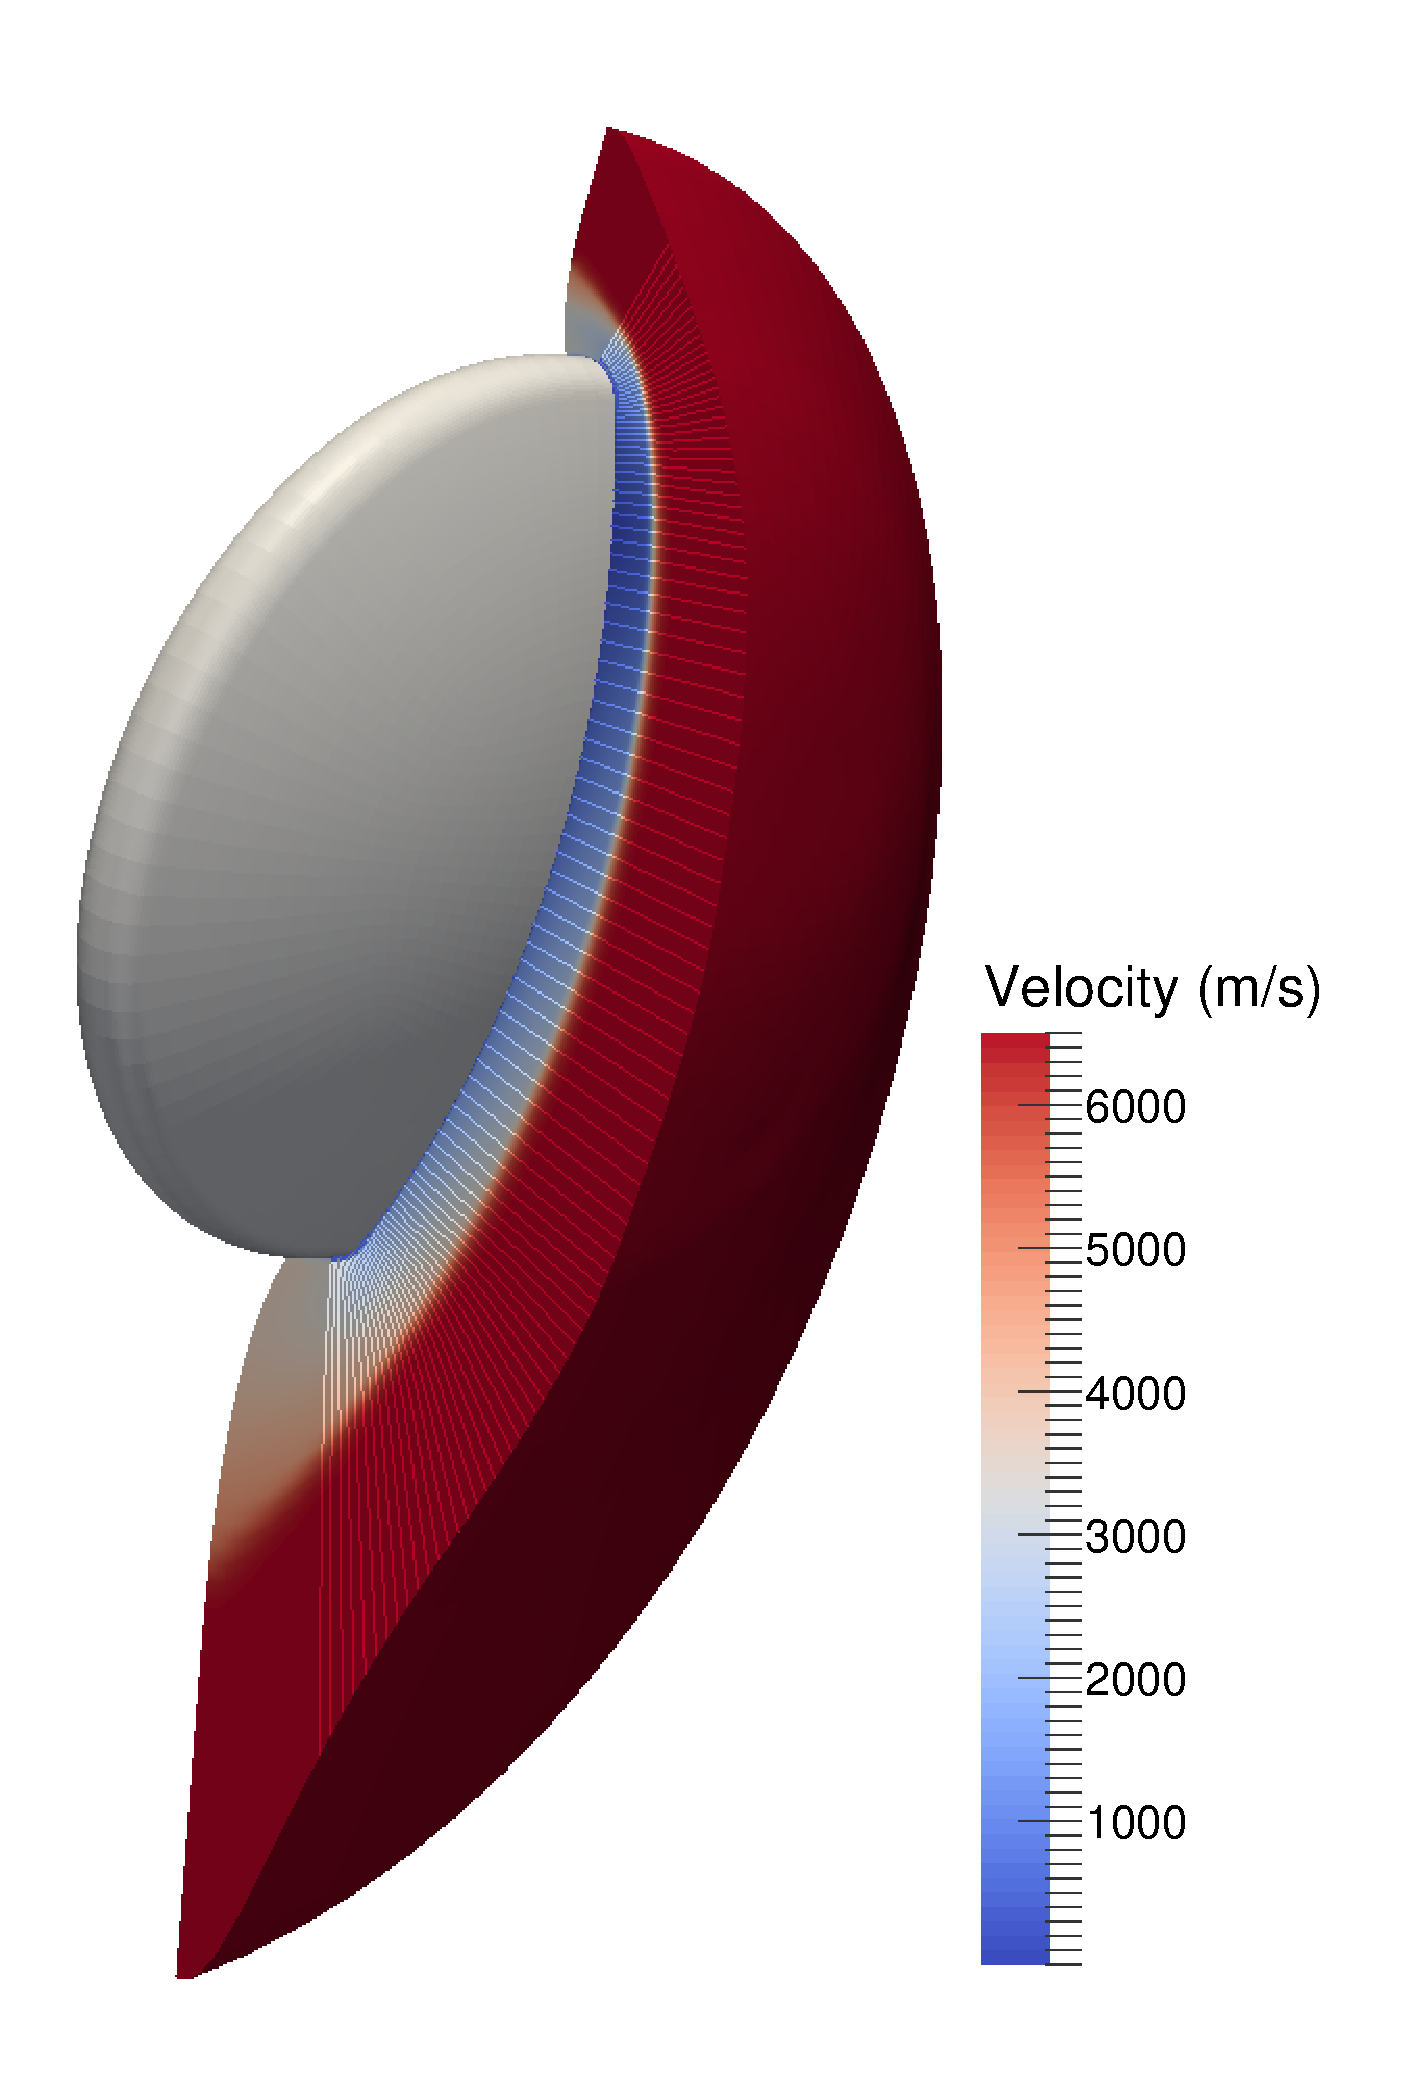
\includegraphics[height=0.92\textheight]{symplanenorm}
  \caption{
    \label{fig:cev_symplane}
    The velocity magnitude on the symmetry plane for the fully laminar
    CEV simulation of interest.
  }
\end{figure}

General boundary layer quantities are plotted in Figure~\ref{fig:cev_summary1}.
Only a few of the plotted quantities are relevant to finding a matching
inviscid base flow.  The ratio of specific heats $\gamma$ and edge Mach number
$\Mach[e]{}$ are taken from the boundary layer edge at distance $\delta$ from
the heat shield surface. The edge-to-wall temperature ratio $T_e/T_w$ captures
the coldness of the wall relative to edge conditions.   When nondimensional
$T_w = 1$ is prescribed as a viscous, isothermal wall condition, the ratio may
be used to fix $T_e$. Though present in the CEV simulations and depicted here,
heat shield curvature and wall blowing are neglected.

\begin{figure}[p]
  \centering
  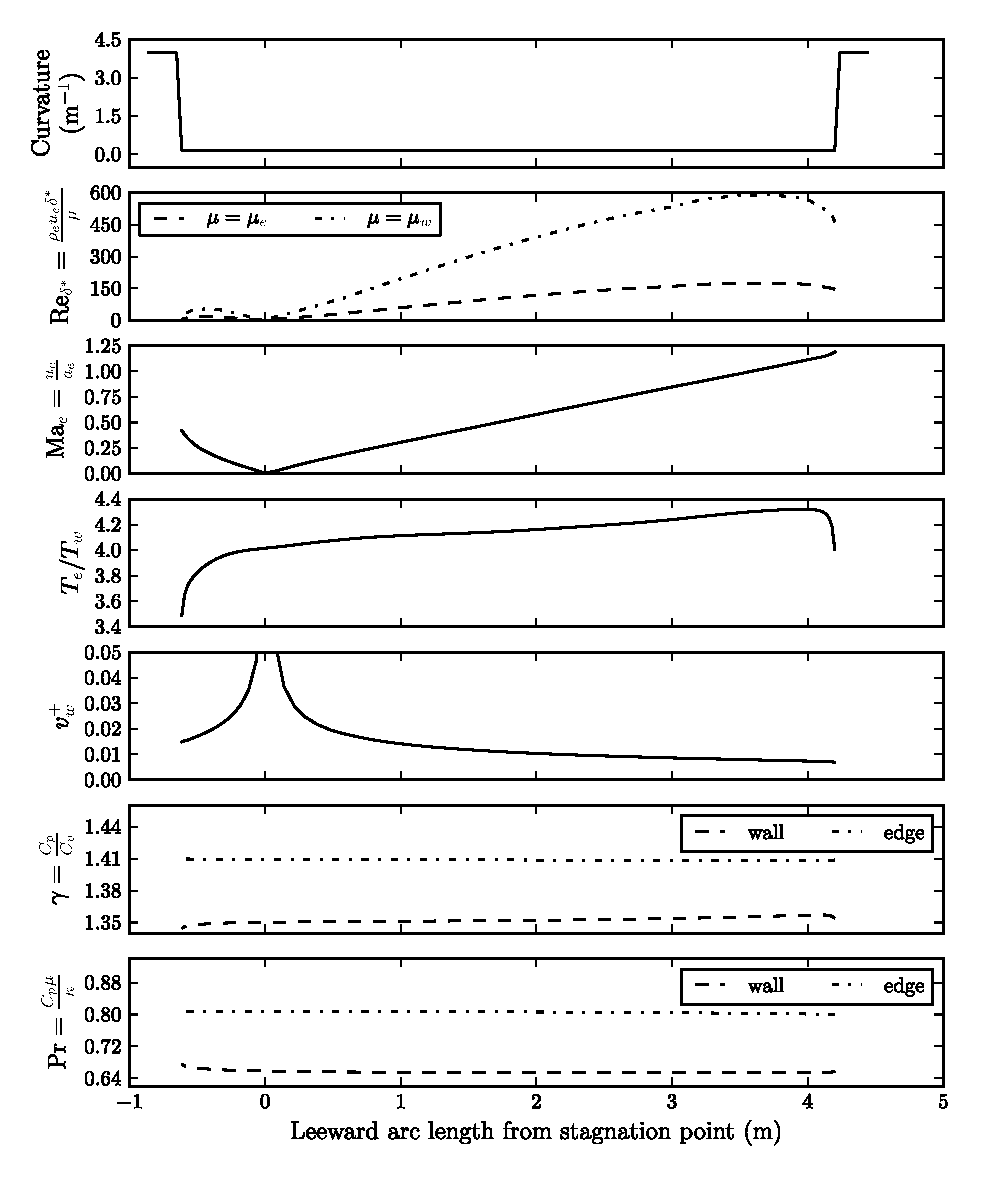
\includegraphics[height=0.92\textheight]{cev_summary1}
  \caption{
    \label{fig:cev_summary1}
    Boundary layer conditions from the fully laminar CEV symmetry plane
  }
\end{figure}

The observed favorable pressure gradient boundary layer nature is quantified in
Figure~\ref{fig:cev_summary_fpg} in a variety of ways.  Of all of these
nondimensional results, $p_{e,\xi}$ is the only quantity with a
directly computable inviscid analog when a target viscous boundary layer
thickness $\delta$ is supplied.  The other nondimensional pressure gradient
parameters, discussed by many authors including
\citet{Sreenivasan1982Laminarescent}, were not adopted for matching purposes as
they require more-complicated flow descriptors like $\delta^\ast$ and $\tau_w$
or the numerically noisy $\frac{\partial\delta}{\partial\xi}$.

\begin{figure}[p]
  \centering
  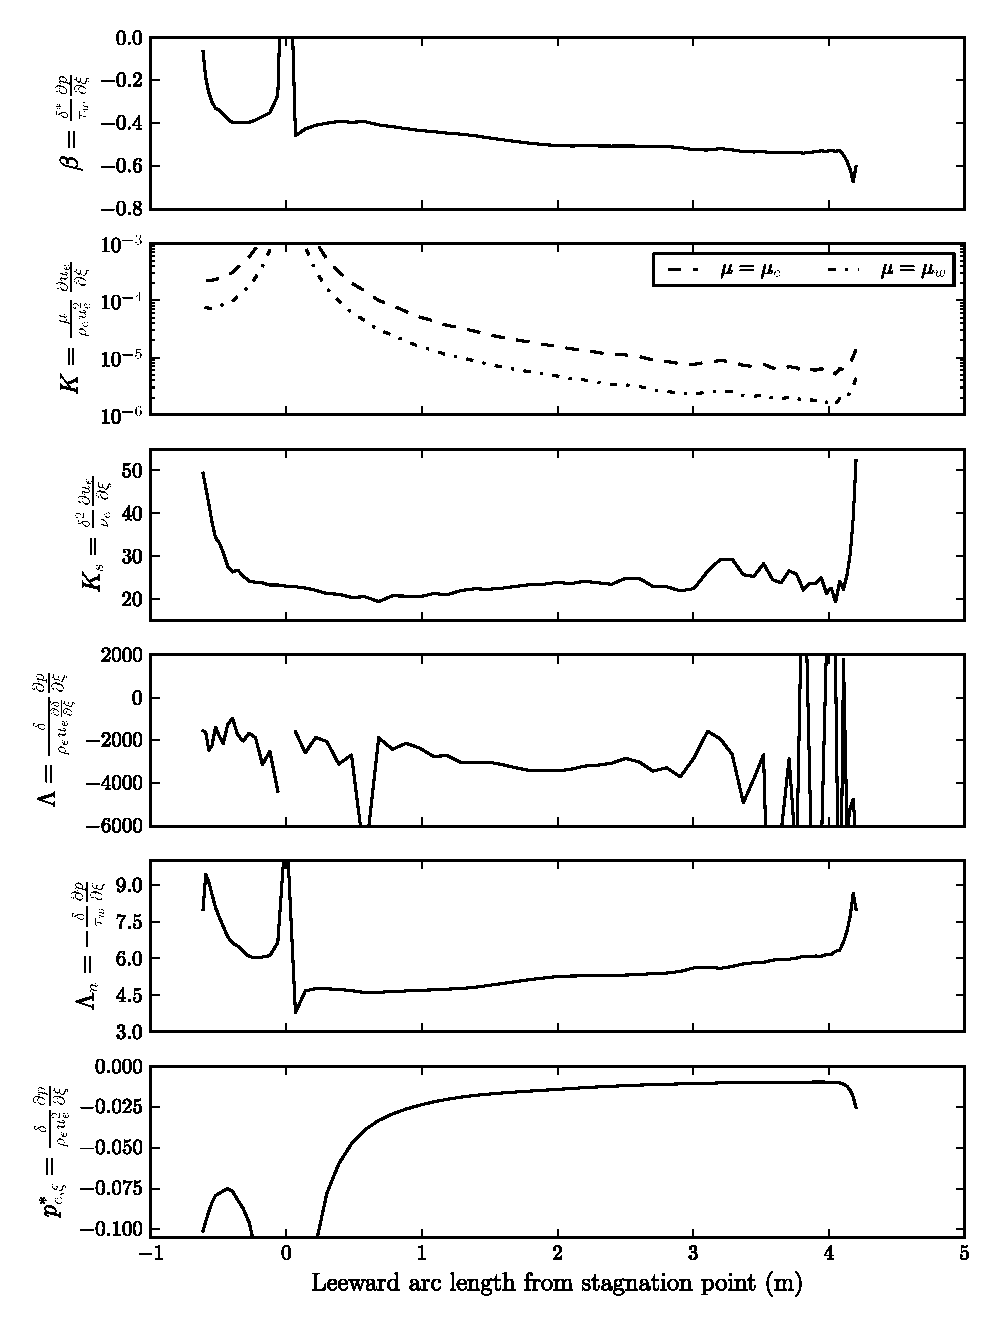
\includegraphics[height=0.92\textheight]{cev_summary_fpg}
  \caption{
    \label{fig:cev_summary_fpg}
    Pressure gradient conditions from the fully laminar CEV symmetry plane.
    Numerical differentiation artifacts are problematic in quantities $\Lambda$
    and $K_s$.
  }
\end{figure}

Conditions $\gamma_e$, $\Mach[e]{}$, $p_{e,\xi}$, and $T_e/T_w$ taken from the
surface-normal rays of Figure~\ref{fig:cev_symplane} were fed into
Listing~\ref{lst:octave_nozzle_match} to produce a family of inviscid base flow
solutions. As these base flows are intended to be used in a simulation with
roughly nondimensional unit thickness and edge density, $\delta=1$ and
$\rho\!\left(R\right)=1$ were held constant.  The CEV-based input data and
computed output at $R=\sqrt{R_0^2+\delta^2}$ are tabulated below.

\clearpage

\begin{centering}
\pgfplotstabletypeset[
  col sep=comma
 ,header=true
 ,clear infinite
 ,begin table=\begin{longtable}
 ,end table=\end{longtable}
 ,every head row/.style={before row=\toprule,after row=\midrule\endhead}
 ,every odd row/.style={before row={\rowcolor[gray]{0.95}}}
 ,columns={dstag,gamma_e,Ma_edge,p_exi,T_ratio,Ma0,R0,u1,p1}
 ,columns/dstag/.style=  {fixed,fixed zerofill,precision=3,dec sep align,column name=Arc length}
 ,columns/gamma_e/.style={fixed,fixed zerofill,precision=4,dec sep align,column name=$\gamma_e$}
 ,columns/Ma_edge/.style={fixed,fixed zerofill,precision=4,dec sep align,column name=$\Mach[e]{}$}
 ,columns/p_exi/.style=  {fixed,fixed zerofill,precision=6,dec sep align,column name=$p_{e,\xi}$}
 ,columns/T_ratio/.style={fixed,fixed zerofill,precision=4,dec sep align,column name=$T_e$}
 ,columns/Ma0/.style=    {fixed,fixed zerofill,precision=4,dec sep align,column name=$\Mach[0]{}$}
 ,columns/R0/.style=     {fixed,fixed zerofill,precision=2,dec sep align,column name=$R_0$}
 ,columns/u1/.style=     {fixed,fixed zerofill,precision=4,dec sep align,column name=$u\!\left(R\right)$}
 ,columns/p1/.style=     {fixed,fixed zerofill,precision=4,dec sep align,column name=$p\!\left(R\right)$}
]{notebooks/cev_laminar.out}
\end{centering}

\newcommand*{\doi}[1]{\href{http://dx.doi.org/\detokenize{#1}}{doi: #1}}
\bibliographystyle{plainnat}
\bibliography{references}

\end{document}
